\documentclass[../../projlab]{subfiles}
\begin{document}

\makeatletter

\ifSubfilesClassLoaded{
	\coverpage{2. Leadás}
	%\renewcommand{\filePath}[1]{./../../ #1}
	\def\filePath[#1]{./../../#1}
}{}

\makeatother

\chapter{Analízis modell kidolgozása 1.}

\markdownInput[shiftHeadings=1]{\subfix{Object-catalog.md}}

%\section{Statikus struktúra diagramok}
%\comment{Az előző alfejezet osztályainak kapcsolatait és publikus metódusait bemutató osztálydiagram(ok). Tipikus hibalehetőségek: csillag-topológia, szigetek.}

%\diagram{docs/img/BMElogo}{Demó}{3cm}

\section{Osztályok leírása}
%\comment{Az előző alfejezetben tárgyalt objektumok felelősségének formalizálása attribútumokká, metódusokká. Csak publikus metódusok szerepelhetnek. Ebben az alfejezetben megjelennek az interfészek, az öröklés, az absztrakt osztályok. Segédosztályokra még mindig nincs szükség. Az osztályok ABC sorrendben kövessék egymást. Interfészek esetén az Interfészek, Attribútumok pontok kimaradnak.}

\subsection{Asteroid}
\begin{class-template-responsibility}
Egy aszteroidát jelöl. Minden példányának létrejöttekor beállítódnak a generátor által a tulajdonságai.
\end{class-template-responsibility}
\begin{class-template-interface}
$\emptyset$
\end{class-template-interface}
\begin{class-template-baseclass}
Entity
\end{class-template-baseclass}
\begin{class-template-attribute}
\classitem{-coreSize:int}{Az aszteroida magjának mérete, ennyi egységnyi nyersanyag bányászható ki belőle a játék elején, és bányászat után ennyi egységnyi item helyezhető vissza bele. }
\classitem{-exploded:bool}{Igaz, ha felrobbant már az aszteroida, hamis, ha nem. }
\classitem{-maxHidingSpace:int}{Maximum ennyi telepes számára van az adott időpillanatban hely az aszteroidában elbújni. Minden telepes sikeres elbújása után csökken ez a szám. }
\classitem{-crustSize:int}{Az aszteroida köpenyének mélysége. Ennyi egységet kell még fúrni benne jelenleg, hogy teljesen átfúrt legyen. Minden fúrás után csökken ez a szám. }
\classitem{-revealed:bool}{Igaz, ha az aszteroida már „fel van fedve” a térképen, tehát rajta vagy bármelyik szomszédján már járt telepes vagy robot. Ellenkező esetben hamis.}
\classitem{-visited:bool}{Igaz, ha az aszteroidán már járt telepes vagy robot, ellenkező esetben hamis.}
\classitem{-hidingVessel:Vessel}{Ha az aszteroidában jelenleg megbújik egy telepes, akkor eltárolja, melyik telepesről van szó. Ha nem bújik benne senki, null értéket tárol.}
\classitem{-inventory:Inventory[1]}{Az aszteroida raktára, ami a magba belehelyezett és jelenleg ott tárolt elemeket tartalmazza. }
\classitem{-neighbours:Asteroid[1..*]}{A szomszédos aszteroidák tárolója.}
\classitem{-resource:Resource[0..1]}{Az aszteroida magjában lévő nyersanyagkészlet. }
\classitem{-stationed:Vessel[0..*]}{Az aszteroidán jelenleg állomásozó járművek tárolója. }
\classitem{-buildings:Building[0..*]}{Az aszteroidára épített (véglegesen elhelyezett) építmények tárolója. }
\end{class-template-attribute}
\begin{class-template-method}
\classitem{+Asteroid(r:Resource):Asteroid}{Az osztály konstruktora.}
\classitem{+Explode()}{Felrobban az aszteroida. Felrobbantja az összes rajta tartózkodó járművet, hozzáférhetetlenné teszi a raktárat és a rajta lévő épületeket, értesíti a szomszédos aszteroidákat a robbanásról. }
\classitem{+ReachableAsteroids():Asteroid}{Tárolja, hogy melyik aszteroidák elérhetőek jelenleg az adott aszteroidából. }
\classitem{+Depart(v:Vessel)}{Egy adott jármű elhagyja az aszteroidát, törlődik az ott tartózkodók közül. }
\classitem{+Arrive(v:Vessel)}{Egy adott jármű érkezik az aszteroidára, regisztrálja az ott tartózkodók közé.}
\classitem{+GetAvailableHidingSpace():int}{Visszaadja, hogy hány telepes számára van még hely elbújásra jelenleg az aszteroidában, attól függően, hogy jelentleg elbújt-e telepes az aszteroidában. }
\classitem{+Reveal()}{Aszteroida felfedése a térképen, amennyiben még nem volt felfedve.  }
\classitem{+Drill()}{Akkor hívódik meg amikor az aszteroida kérgén lévő lyukat akarják mélyíteni.}
\classitem{+Mine():Item}{Akkor hívódik meg amikor az aszteroidából akarnak nyersanyagot kibányászni.}
\classitem{+Hide(v:Vessel):bool}{Az aszteroidában megpróbál elbújni egy jármű. Igazat ad vissza ha el tud bújni, hamisat ha nem.}
\classitem{+Exit(v:Vessel)}{Az adott jármű előbújik az aszteroidából.}
\classitem{+AddBuilding(b:Building)}{Hozzáad egy új épületet az aszteroidához.}
\classitem{+PlaceItem(i:Item):bool}{Elem belehelyezése a raktárba. Sikeres behelyezés után igazzal tér vissza, sikertelen művelet után hamissal tér vissza. }
\classitem{+AddNeigbour(a:Asteroid)}{Új szomszéd hozzáadása. }
\classitem{+GetInventory():return:Inventory}{Visszaadja az aszteroida raktárát. }
\classitem{+SolarFlare()}{Napvihar esetén hívódik meg minden entitáson, az aszteroidákon nem történik művelet ilyenkor.}
\end{class-template-method}


\subsection{Building}
\begin{class-template-responsibility}
Az épülettípusok közös ősosztálya. 
\end{class-template-responsibility}
\begin{class-template-interface}
$\emptyset$
\end{class-template-interface}
\begin{class-template-baseclass}
$\emptyset$
\end{class-template-baseclass}
\begin{class-template-attribute}
\classitem{-asteroid:Asteroid[1]}{Az épület lerakási helye (aszteroida).}
\classitem{-position:BuildingPlace}{Azt jelöli,hogy az épület hol helyezkedik el az aszteroidán.}
\end{class-template-attribute}
\begin{class-template-method}
\classitem{+Explode()}{Akkor hívódik meg, ha valamilyen okból az épület megsemmisül.}
\classitem{+GetRoutes():Asteroid}{Az ebből az épületből elérhető extra aszteroidákat adja vissza.}
\classitem{+Building(a:Asteroid):Building}{Az osztály konstruktora, beállítja az aktuális tartózkodási helyet. }
\end{class-template-method}


\subsection{Coal}
\begin{class-template-responsibility}
A szén reprezentálására szolgál az Inventory-ban.
\end{class-template-responsibility}
\begin{class-template-interface}
$\emptyset$
\end{class-template-interface}
\begin{class-template-baseclass}
Item
\end{class-template-baseclass}
\begin{class-template-attribute}
\item[] $\emptyset$
\end{class-template-attribute}
\begin{class-template-method}
\classitem{+Satisfies(i:Item):bool}{Meghatározza, hogy az átadott Item használható-e a jelenlegi helyett.}
\end{class-template-method}


\subsection{CoalResource}
\begin{class-template-responsibility}
Egy adott aszteroidában tárolt szén, adott számú egységgel rendelkező, bányászással kinyerhető nyersanyagkészletért felel. 
\end{class-template-responsibility}
\begin{class-template-interface}
$\emptyset$
\end{class-template-interface}
\begin{class-template-baseclass}
Resource
\end{class-template-baseclass}
\begin{class-template-attribute}
\item[] $\emptyset$
\end{class-template-attribute}
\begin{class-template-method}
\classitem{+Satisfies(r:Resource):bool}{Meghatározza, hogy az átadott Resource használható-e a szén helyett.}
\end{class-template-method}


\subsection{Engine}
\begin{class-template-responsibility}
A program indításáért, egy játékfolyam bezárásáért felelős osztály. 
\end{class-template-responsibility}
\begin{class-template-interface}
$\emptyset$
\end{class-template-interface}
\begin{class-template-baseclass}
$\emptyset$
\end{class-template-baseclass}
\begin{class-template-attribute}
\item[] $\emptyset$
\end{class-template-attribute}
\begin{class-template-method}
\classitem{+StartApplication()}{A program indítása.}
\classitem{+StartGame()}{Egy új játék kezdése.}
\classitem{+EndGame()}{Játékmenetek befejezése. }
\end{class-template-method}


\subsection{Entity}
\begin{class-template-responsibility}
Egy adott entitás ( vizuális megjelenítéssel rendelkező játékelem) osztálya. 
\end{class-template-responsibility}
\begin{class-template-interface}
$\emptyset$
\end{class-template-interface}
\begin{class-template-baseclass}
$\emptyset$
\end{class-template-baseclass}
\begin{class-template-attribute}
\classitem{Not definedscene:Scene[1]}{A játéktér tárolója. }
\end{class-template-attribute}
\begin{class-template-method}
\classitem{+RoundEnd()}{Akkor hívódik meg, ha az adott körben már minden játékos lépett. A robotok ezt használják például a mozgásra.}
\classitem{+GetScene():Scene}{A játéktér getter-e. }
\classitem{+SolarFlare()}{Napviharról értesíti az egységet.}
\end{class-template-method}


\subsection{GameManager}
\begin{class-template-responsibility}
A játék menetének irányításáért felelős osztály. 
\end{class-template-responsibility}
\begin{class-template-interface}
$\emptyset$
\end{class-template-interface}
\begin{class-template-baseclass}
$\emptyset$
\end{class-template-baseclass}
\begin{class-template-attribute}
\classitem{-currentPlayer:}{The player who is taking the turn currently}
\classitem{-selectedVessel:Vessel}{Az aktuálisan irányítható jármű (akit a soron lévő játékos jelenleg irányít). }
\classitem{-sunDistance:int}{A Naptól való aktuális távolság. }
\classitem{-allPlayers:Player[1..*]}{A játék játékosainak listája. }
\classitem{-asteroids:Asteroid[1..*]}{A játékban szereplő aszteroidák listája. }
\classitem{-gameEnded:bool}{Jelzi, hogy a játék befejeződött-e már.}
\classitem{-settlers:SpaceShip}{A játék telepeseinek tárolója. }
\classitem{-currentPlayer:Player[1]}{A jelenleg aktív játékos, aki éppen tudja mozgatni a telepesit.}
\classitem{-scene:Scene}{Az adott játékhoz tartozó játéktér. }
\end{class-template-attribute}
\begin{class-template-method}
\classitem{+InitGame()}{A játékmenet inicializálásáért felel. }
\classitem{+AddPlayer(p:Player)}{Új játékos hozzáadása. }
\classitem{+StartGame()}{Új játék indításáért felel. }
\classitem{+TakeTurn()}{Egy játékos aktuális köre - ekkor van lehetősége irányítani a járműveit egyesével. }
\classitem{+EndGame()}{Aktuális játék befejezése. }
\classitem{-GenerateScene()}{Játék inicializálás során a játéktér elemeinek inicializálása.}
\classitem{-GenerateNewResource():Resource}{Új nyersanyag generálása, inicializálás folyamata során használjuk fel. }
\classitem{-GenerateAsteroids()}{Az aszteroidamező inicializálása, játék inicializálás során hozzuk létre.}
\classitem{+IsSunStormActive():bool}{Visszaadja, hogy jelenleg napviharban van-e az aszteroidamező. }
\end{class-template-method}


\subsection{Ice}
\begin{class-template-responsibility}
A jég reprezentálására szolgál az Inventory-ban.
\end{class-template-responsibility}
\begin{class-template-interface}
$\emptyset$
\end{class-template-interface}
\begin{class-template-baseclass}
Item
\end{class-template-baseclass}
\begin{class-template-attribute}
\item[] $\emptyset$
\end{class-template-attribute}
\begin{class-template-method}
\classitem{+Satisfies(i:Item):bool}{Meghatározza, hogy az átadott Item használható-e a jelenlegi helyett.}
\end{class-template-method}


\subsection{IceResource}
\begin{class-template-responsibility}
Egy adott aszteroidában tárolt jég, adott számú egységgel rendelkező, bányászással kinyerhető nyersanyagkészletért felel. 
\end{class-template-responsibility}
\begin{class-template-interface}
$\emptyset$
\end{class-template-interface}
\begin{class-template-baseclass}
Resource
\end{class-template-baseclass}
\begin{class-template-attribute}
\item[] $\emptyset$
\end{class-template-attribute}
\begin{class-template-method}
\classitem{+Satisfies(r:Resource):bool}{Meghatározza, hogy az átadott Resource használható-e a jég helyett.}
\classitem{+NearSun()}{Napközelben a nyersanyag típusának megfelelő műveletet hajt végre.  A jég körönként 1 egységnyi sebességgel párolog.}
\end{class-template-method}


\subsection{Inventory}
\begin{class-template-responsibility}
Egy aszteroidán vagy telepesnél található kinyert nyersanyagok (itemek) tárolója.
Ezt az osztályt használja az Aszteroida illetve a telepesk ürhejója a megszerzett nyersanyagok tárolására.
\end{class-template-responsibility}
\begin{class-template-interface}
$\emptyset$
\end{class-template-interface}
\begin{class-template-baseclass}
$\emptyset$
\end{class-template-baseclass}
\begin{class-template-attribute}
\classitem{-size:int}{A tároló kapacitása. }
\classitem{-items:Item[0..*]}{A tárolóban aktuálisan tárolt elemek. }
\end{class-template-attribute}
\begin{class-template-method}
\classitem{+InsertItem(item:Item):bool}{Új elem hozzáadása a tárolóhoz, amennyiben van benne szabad hely (kapacitás).  Sikeres művelet esetén igaz, sikertelen művelet esetén hamis visszatérési értéke van. }
\classitem{+RemoveItem(item:Item)}{Elem eltávolítása a tárolóból. }
\classitem{+TryInsertItem(item:Item):bool}{Ellenőrzi, hogy az adott elem elméletileg belehelyezhető-e a raktárba. }
\classitem{+getItems():Item}{Visszatér az inventory-ban találtahó item-ek listájával.}
\end{class-template-method}


\subsection{Iron}
\begin{class-template-responsibility}
 A Vas reprezentálására szolgál az Inventory-ban.
\end{class-template-responsibility}
\begin{class-template-interface}
$\emptyset$
\end{class-template-interface}
\begin{class-template-baseclass}
Item
\end{class-template-baseclass}
\begin{class-template-attribute}
\item[] $\emptyset$
\end{class-template-attribute}
\begin{class-template-method}
\classitem{+Satisfies(i:Item):bool}{Meghatározza, hogy az átadott Item használható-e a jelenlegi helyett.}
\end{class-template-method}


\subsection{IronResource}
\begin{class-template-responsibility}
Egy adott aszteroidában tárolt vas, adott számú egységgel rendelkező, bányászással kinyerhető nyersanyagkészletért felel. 
\end{class-template-responsibility}
\begin{class-template-interface}
$\emptyset$
\end{class-template-interface}
\begin{class-template-baseclass}
Resource
\end{class-template-baseclass}
\begin{class-template-attribute}
\item[] $\emptyset$
\end{class-template-attribute}
\begin{class-template-method}
\classitem{+Satisfies(r:Resource):bool}{Meghatározza, hogy az átadott Resource használható-e a vas helyett.}
\end{class-template-method}


\subsection{Item}
\begin{class-template-responsibility}
A már kibányászott nyersanyagok hordozható elemekké válnak, ebben a formában tárolja őket az osztály. Egy típusú, adott mennyiségű azonos elemet, illetve hordozható épületet (pl. teleportkapu-pár) tárol.
\end{class-template-responsibility}
\begin{class-template-interface}
$\emptyset$
\end{class-template-interface}
\begin{class-template-baseclass}
$\emptyset$
\end{class-template-baseclass}
\begin{class-template-attribute}
\classitem{-amount:int}{Az elem darabszámát tárolja. }
\end{class-template-attribute}
\begin{class-template-method}
\classitem{+Satisfies(i:Item):bool}{Meghatározza, hogy az átadott Item használható-e a jelenlegi helyett.
}
\classitem{+Reduce(a:int)}{A megadott számmal csökkenti az adott Item méretét (számosságát), amennyiben ez lehetséges.}
\classitem{+Activate(s:SpaceShip)}{Aktiválható tárgyaknál( pl.Teleport kapu) használt függvény. Alapból nem csinál semmit.}
\end{class-template-method}


\subsection{Player}
\begin{class-template-responsibility}
Egy adott játékos reprezentációja. 
\end{class-template-responsibility}
\begin{class-template-interface}
$\emptyset$
\end{class-template-interface}
\begin{class-template-baseclass}
$\emptyset$
\end{class-template-baseclass}
\begin{class-template-attribute}
\classitem{-name:string}{A játékos neve.}
\classitem{-searching\_for:Resource[1]}{}
\end{class-template-attribute}
\begin{class-template-method}
\item[] $\emptyset$
\end{class-template-method}


\subsection{Recipe}
\begin{class-template-responsibility}
A telepesek által elkészíthető receptekért felel. Egy recept adott számú kibányászott nyersanyag (elem) felhasználásával elkészített dolgok pontos hozzávalóit, és az elkészült eredmény típusát tárolja. 
\end{class-template-responsibility}
\begin{class-template-interface}
$\emptyset$
\end{class-template-interface}
\begin{class-template-baseclass}
$\emptyset$
\end{class-template-baseclass}
\begin{class-template-attribute}
\classitem{-input:Item[1..*]}{Az aktuális recepthez szükséges hozzávalók tárolása. }
\end{class-template-attribute}
\begin{class-template-method}
\classitem{+CanCraft(inv:Inventory, a:Asteroid):bool}{Meghatározza, hogy egy adott raktárban és aszteroidán lévő kibányászott nyersanyagkészlet elegendő-e az adott recept elkészítéséhez. }
\classitem{+Craft(inv:Inventory, a:Asteroid)}{Akkor hívódik meg ha ténylegesen le akarjuk gyártani ezt a receptet.}
\classitem{Not definedMakeResult(inv:Inventory, a:Asteroid)}{Létrehozza a kívánt terméket a receptből.}
\end{class-template-method}


\subsection{Resource}
\begin{class-template-responsibility}
Egy adott aszteroidában tárolt egy fajta (egy konkrét típusú), adott számú egységgel rendelkező, bányászással kinyerhető nyersanyagkészletért felel. 
\end{class-template-responsibility}
\begin{class-template-interface}
$\emptyset$
\end{class-template-interface}
\begin{class-template-baseclass}
$\emptyset$
\end{class-template-baseclass}
\begin{class-template-attribute}
\classitem{-amount:int}{A játék adott pillanatában ennyi egységnyi nyersanyag bányászható még ki az aszteroidából. }
\end{class-template-attribute}
\begin{class-template-method}
\classitem{+Mine():Item}{Egy egység nyersanyag kinyerése bányászattal, amennyiben ez lehetséges (rendelkezésre áll elég nyersanyag). Ekkor egy kibányászott megfelelő elemmel tér vissza.}
\classitem{+NearSun()}{Napközelben a nyersanyag típusának megfelelő műveletet hajt végre. Különleges képességekkel nem rendelkező nyersanyagok esetén nem hajt végre műveletet.  }
\classitem{+Satisfies(r:Resource):bool}{Meghatározza, hogy az átadott Item használható-e a jelenlegi helyett.}
\end{class-template-method}


\subsection{Robot}
\begin{class-template-responsibility}
Egy speciális jármű, a robot tevékenységeit, tulajdonságait tartalmazza.
\end{class-template-responsibility}
\begin{class-template-interface}
$\emptyset$
\end{class-template-interface}
\begin{class-template-baseclass}
Entity \baseclass Vessel
\end{class-template-baseclass}
\begin{class-template-attribute}
\item[] $\emptyset$
\end{class-template-attribute}
\begin{class-template-method}
\classitem{+Robot(p:Player, a:Asteroid):Robot}{Az osztály konstruktora, beállítja az őt kezelő játékost illetve aszteroidát. }
\classitem{+GetHidingSpaceRequirement():int}{A robotok által az aszteroida magjában elfoglalt hely nagyságát adja vissza. Korlátlan mennyiségű robot elfér, tehát 0 az értéke. }
\end{class-template-method}


\subsection{RobotRecipe}
\begin{class-template-responsibility}
Robotok legyártásáért feleős osztály.
\end{class-template-responsibility}
\begin{class-template-interface}
$\emptyset$
\end{class-template-interface}
\begin{class-template-baseclass}
Recipe
\end{class-template-baseclass}
\begin{class-template-attribute}
\item[] $\emptyset$
\end{class-template-attribute}
\begin{class-template-method}
\item[] $\emptyset$
\end{class-template-method}


\subsection{Scene}
\begin{class-template-responsibility}
Az entitások összességének összefogásáért felelős osztály. 
\end{class-template-responsibility}
\begin{class-template-interface}
$\emptyset$
\end{class-template-interface}
\begin{class-template-baseclass}
$\emptyset$
\end{class-template-baseclass}
\begin{class-template-attribute}
\classitem{Not definedentities:Entity[1..*]}{A játékban szereplő összes entitás tárolója. }
\classitem{-manager:GameManager}{Az aktuális játékmenet. }
\end{class-template-attribute}
\begin{class-template-method}
\classitem{+AddEntity(e:Entity)}{Új entitás hozzáadása a játékmenethez.}
\classitem{+RoundEnded()}{Az összes entitás RoundEnd() metódusát meghívja, befejezi az adott kört. }
\classitem{+GetManager():GameManager}{A manager attribútum getter-e. }
\classitem{+SolarFlare()}{A napviharról szóló értesítést továbbítja az Entity felé}
\end{class-template-method}


\subsection{SpaceShip}
\begin{class-template-responsibility}
A telepesekért felelős osztály.
\end{class-template-responsibility}
\begin{class-template-interface}
$\emptyset$
\end{class-template-interface}
\begin{class-template-baseclass}
Entity \baseclass Vessel
\end{class-template-baseclass}
\begin{class-template-attribute}
\classitem{-lastPlacedGate:TeleportGate}{Az utoljára lehelyezett kapu referenciája. Arra használjuk hogy a telepes által lerakott kapu párokat össze lehessen kötni.}
\classitem{-inventory:Inventory[1]}{A telepes által folyamatosan hordozott raktár. }
\end{class-template-attribute}
\begin{class-template-method}
\classitem{+SpaceShip(p:Player, a:Asteroid):SpaceShip}{Az osztály konstruktora, beállítja az őt kezelő játékost illetve aszteroidát. }
\classitem{+GetHidingSpaceRequirement():int}{A telepesek által az aszteroida magjában elfoglalt hely nagyságát adja vissza. }
\classitem{+Mine()}{Teljesen átfúrt, nem üres magú aszteroidán való tartózkodás esetén a telepes egy egységet kibányászik az ott található nyersanyagból. Az így keletkező elem a telepes raktárába kerül.  Ha sikertelen a művelet (nem teljesülnek a feltételek), nem történik művelet. }
\classitem{+Craft(recipe:Recipe)}{A telepes az aktuálisan rendelkezésére álló elemekből egy "receptet" készít.  A felhasznált elemek elhasználódnak, törlődnek a raktárból. }
\classitem{+PlaceItem(i:Item):bool}{Elem belehelyezése az aktuális aszteroidába, amin tartózkodik. Sikeres behelyezés után igazzal tér vissza, a saját raktárból eltávolítja az elemet. Sikertelen művelet után hamissal tér vissza. }
\classitem{+ActivateItem(i:Item)}{A megadott tárgyon hív egy Activate()-et}
\end{class-template-method}


\subsection{SpaceStation}
\begin{class-template-responsibility}
A játékosok által megépítendő űrállomás épület típust jelöli. Speciális tulajdonsága, hogy amikor megépül akkor a játék befejeződik.
\end{class-template-responsibility}
\begin{class-template-interface}
$\emptyset$
\end{class-template-interface}
\begin{class-template-baseclass}
Building
\end{class-template-baseclass}
\begin{class-template-attribute}
\item[] $\emptyset$
\end{class-template-attribute}
\begin{class-template-method}
\classitem{+SpaceStation(a:Asteroid):SpaceStation}{Meghívódik ha az adott aszteroidán egy űrállomás épült. Ekkor a játék befejeződik.}
\classitem{+Explode(a:Asteroid)}{Az űrállomás felrobbanásakor hívódik meg.  Ez gyakorlatban sosem fog megtörténni, hiszen amint felépül az űrállomás, a játékot megnyerik. }
\classitem{+GetRoutes():Asteroid}{Az ebből az épületből elérhető extra aszteroidákat adja vissza.}
\end{class-template-method}


\subsection{SpaceStationRecipe}
\begin{class-template-responsibility}
Aszteroidákra elhelyezhető épületek receptjeiért felelős osztály. 
\end{class-template-responsibility}
\begin{class-template-interface}
$\emptyset$
\end{class-template-interface}
\begin{class-template-baseclass}
Recipe
\end{class-template-baseclass}
\begin{class-template-attribute}
\item[] $\emptyset$
\end{class-template-attribute}
\begin{class-template-method}
\item[] $\emptyset$
\end{class-template-method}


\subsection{TeleportGate}
\begin{class-template-responsibility}
A teleportkapukat reprezentáló osztály.
\end{class-template-responsibility}
\begin{class-template-interface}
$\emptyset$
\end{class-template-interface}
\begin{class-template-baseclass}
Building
\end{class-template-baseclass}
\begin{class-template-attribute}
\item[] $\emptyset$
\end{class-template-attribute}
\begin{class-template-method}
\classitem{+GetRoutes():Asteroid}{Visszaadja az ebből a kapuból elérhető extra aszteroidákat.
}
\classitem{+PairDestroyed()}{Akkor hívódik meg ha a párja megsemmisül és ezáltal ez az oldal deaktiválódik.}
\classitem{+Explode(a:Asteroid)}{Akkor hívódik meg ha az épület felrobban. Ekkor szól a szomszédjának is a PairDestroyed() fügvénnyel.}
\end{class-template-method}


\subsection{TeleportGateItem}
\begin{class-template-responsibility}
Teleport kapu amikor még a telepesnél van.
\end{class-template-responsibility}
\begin{class-template-interface}
$\emptyset$
\end{class-template-interface}
\begin{class-template-baseclass}
Item
\end{class-template-baseclass}
\begin{class-template-attribute}
\item[] $\emptyset$
\end{class-template-attribute}
\begin{class-template-method}
\classitem{+Satisfies(i:Item):bool}{Meghatározza, hogy az átadott Item használható-e a jelenlegi helyett.}
\classitem{+Activate(s:SpaceShip)}{A teleportkapuk lehelyezését végző függvény.}
\end{class-template-method}


\subsection{TeleportGateRecipe}
\begin{class-template-responsibility}
Teleportkapu-párok elkészítéséhez szükséges speciális recept típus. 
\end{class-template-responsibility}
\begin{class-template-interface}
$\emptyset$
\end{class-template-interface}
\begin{class-template-baseclass}
Recipe
\end{class-template-baseclass}
\begin{class-template-attribute}
\classitem{-result:TeleportGate}{A sikeres készítés után ilyen típusú eredményhez ("elemhez") lehet hozzájutni. }
\classitem{-amount:int}{Az elkészült dolog mennyisége (egyszerre hány egység készül el belőle)}
\end{class-template-attribute}
\begin{class-template-method}
\item[] $\emptyset$
\end{class-template-method}


\subsection{Titan}
\begin{class-template-responsibility}
A titán reprezentálására szolgál az Inventory-ban
\end{class-template-responsibility}
\begin{class-template-interface}
$\emptyset$
\end{class-template-interface}
\begin{class-template-baseclass}
Item
\end{class-template-baseclass}
\begin{class-template-attribute}
\item[] $\emptyset$
\end{class-template-attribute}
\begin{class-template-method}
\classitem{+Satisfies(i:Item):bool}{Meghatározza, hogy az átadott Item használható-e a jelenlegi helyett.}
\end{class-template-method}


\subsection{TitaniumResource}
\begin{class-template-responsibility}
Egy adott aszteroidában tárolt titán, adott számú egységgel rendelkező, bányászással kinyerhető nyersanyagkészletért felel. 
\end{class-template-responsibility}
\begin{class-template-interface}
$\emptyset$
\end{class-template-interface}
\begin{class-template-baseclass}
Resource
\end{class-template-baseclass}
\begin{class-template-attribute}
\item[] $\emptyset$
\end{class-template-attribute}
\begin{class-template-method}
\classitem{+Satisfies(r:Resource):bool}{Meghatározza, hogy az átadott Resource használható-e a titán helyett.}
\end{class-template-method}


\subsection{Uranium}
\begin{class-template-responsibility}
Az uránium reprezentálására szolgál az Inventory-ban.
\end{class-template-responsibility}
\begin{class-template-interface}
$\emptyset$
\end{class-template-interface}
\begin{class-template-baseclass}
Item
\end{class-template-baseclass}
\begin{class-template-attribute}
\item[] $\emptyset$
\end{class-template-attribute}
\begin{class-template-method}
\classitem{+Satisfies(i:Item):bool}{Meghatározza, hogy az átadott Item használható-e a jelenlegi helyett.}
\end{class-template-method}


\subsection{UraniumResource}
\begin{class-template-responsibility}
Egy adott aszteroidában tárolt urán, adott számú egységgel rendelkező, bányászással kinyerhető nyersanyagkészletért felel. 
\end{class-template-responsibility}
\begin{class-template-interface}
$\emptyset$
\end{class-template-interface}
\begin{class-template-baseclass}
Resource
\end{class-template-baseclass}
\begin{class-template-attribute}
\item[] $\emptyset$
\end{class-template-attribute}
\begin{class-template-method}
\classitem{+Satisfies(r:Resource):bool}{Meghatározza, hogy az átadott Resource használható-e uránium helyett.}
\classitem{+NearSun()}{Napközelben a nyersanyag típusának megfelelő műveletet hajt végre.  Az uránium, ha megfúrt aszteroidában van, akkor felrobban.}
\end{class-template-method}


\subsection{Vessel}
\begin{class-template-responsibility}
Egy-egy járműért (pl. telepes vagy robot) felelős osztály. 
\end{class-template-responsibility}
\begin{class-template-interface}
$\emptyset$
\end{class-template-interface}
\begin{class-template-baseclass}
Entity
\end{class-template-baseclass}
\begin{class-template-attribute}
\classitem{-isHidden:bool}{Ha jelenleg el van bújva az aszteroidájában, igaz, ellenkező esetben hamis. }
\classitem{-currentAsteroid:Asteroid[1]}{Az aktuális tartózkodási helyének (aszteroida) tárolására szolgál. }
\classitem{-owner:Player[1]}{Tárolja, hogy melyik játékos irányítja az járművet.}
\end{class-template-attribute}
\begin{class-template-method}
\classitem{+Vessel(p:Player, a:Asteroid):Vessel}{Az osztály konstruktora, beállítja az őt kezelő játékost illetve aszteroidát. }
\classitem{+Hide()}{Belebújik az adott aszteroidába, ha van benne elegendő hely. Ha nincsen, az aszteroida felszínén marad. }
\classitem{+Drill()}{Fúr egy egységnyit az aszteroida köpenyéből, ha még nincs teljesen átfúrva. Ha át van fúrva, nem történik művelet.}
\classitem{+Move(a:Asteroid)}{Az jármű átlép egy szomszédos aszteroidára. }
\classitem{+GetHidingSpaceRequirement():int}{Absztrakt metódus, leszármazottól függően más értéket ad vissza. Meghatározza, hogy ha az adott jármű el szeretne bújni egy aszteroidában, mennyi helyre van hozzá szüksége. }
\classitem{+Explode()}{Felrobban  a jármű (egy aszteroida robbanásának hatására). }
\classitem{+ExitHiding()}{A jármű kibújik az aszteroida magjából, ha el volt bújva benne. Ha nem, nem történik művelet. }
\classitem{+AsteroidExploded()}{A jelenlegi aszeroida ezen keresztül szól a telep/robot-nak, hogy felrobbant.}
\classitem{+SolarFlare()}{}
\end{class-template-method}




%\begin{class-template-statechart}
%    A belső működéshez tartozó állapotgép
%    \diagram{docs/img/BMElogo}{Az osztály állapotváltozásai}{3cm}
%\end{class-template-statechart}

\section{Statikus struktúra diagramok}
%\comment{Az előző alfejezet osztályainak kapcsolatait és publikus metódusait bemutató osztálydiagram(ok). Tipikus hibalehetőségek: csillag-topológia, szigetek.}
\begin{figure}[H]
	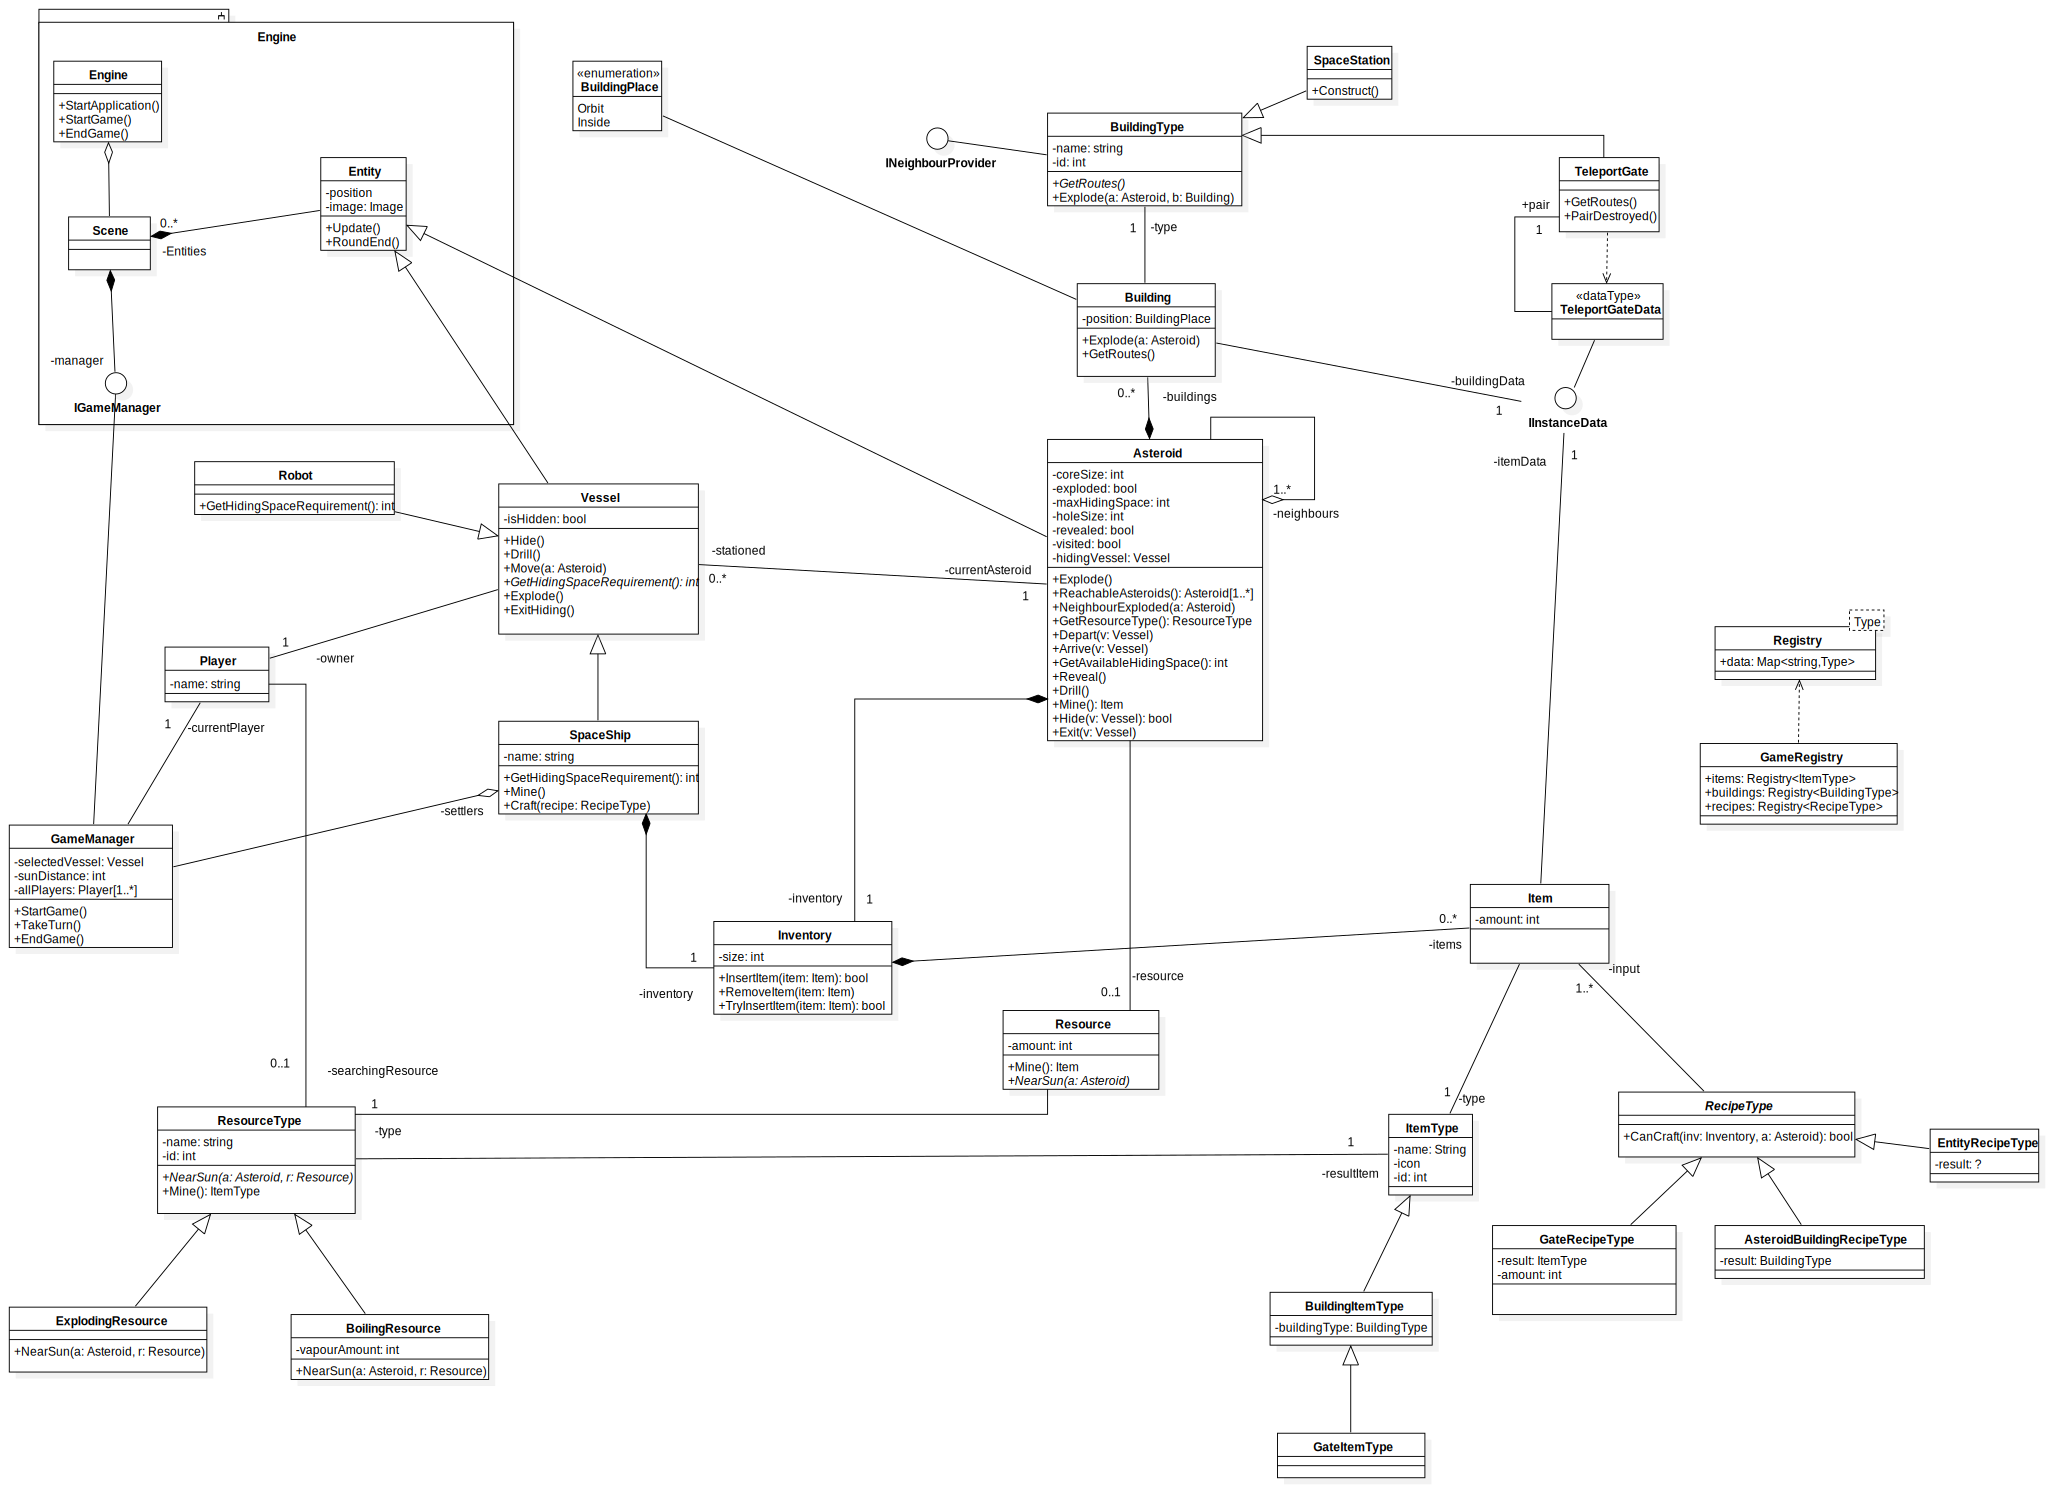
\includegraphics[width=1\textwidth]{docs/2_Project/svg/Design Model!Classes_1.png}
	\centering
\end{figure}

\section{Szekvencia diagramok}
%\comment{Inicializálásra, use-case-ekre, belső működésre. Konzisztens kell legyen az előző alfejezettel. Minden metódus, ami ott szerepel, fel kell tűnjön valamelyik szekvenciában. Minden metódusnak, ami szekvenciában szerepel, szereplnie kell a valamelyik osztálydiagramon.}
%\diagram{docs/img/BMElogo}{Szekvencia1}{3cm}
\begin{figure}[H]
	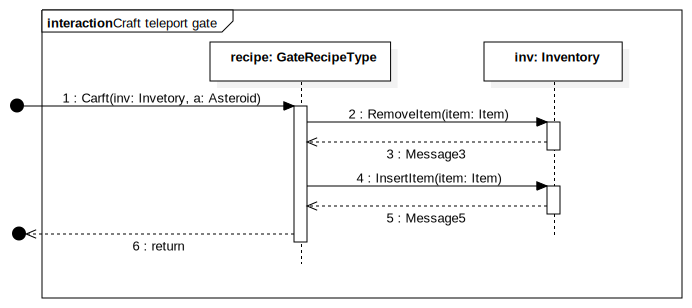
\includegraphics[width=1\textwidth]{docs/2_Project/svg/Design Model!Crafting!Craft teleport gate!Craft teleport gate_19.png}
	\centering
\end{figure}

\begin{figure}[H]
	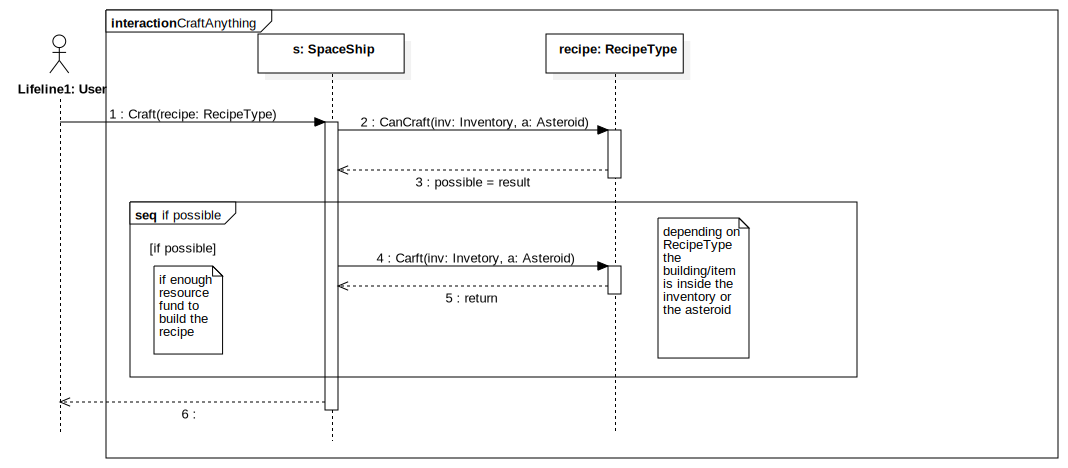
\includegraphics[width=1\textwidth]{docs/2_Project/svg/Design Model!Crafting!Craft!CraftAnything_18.png}
	\centering
\end{figure}

\begin{figure}[H]
	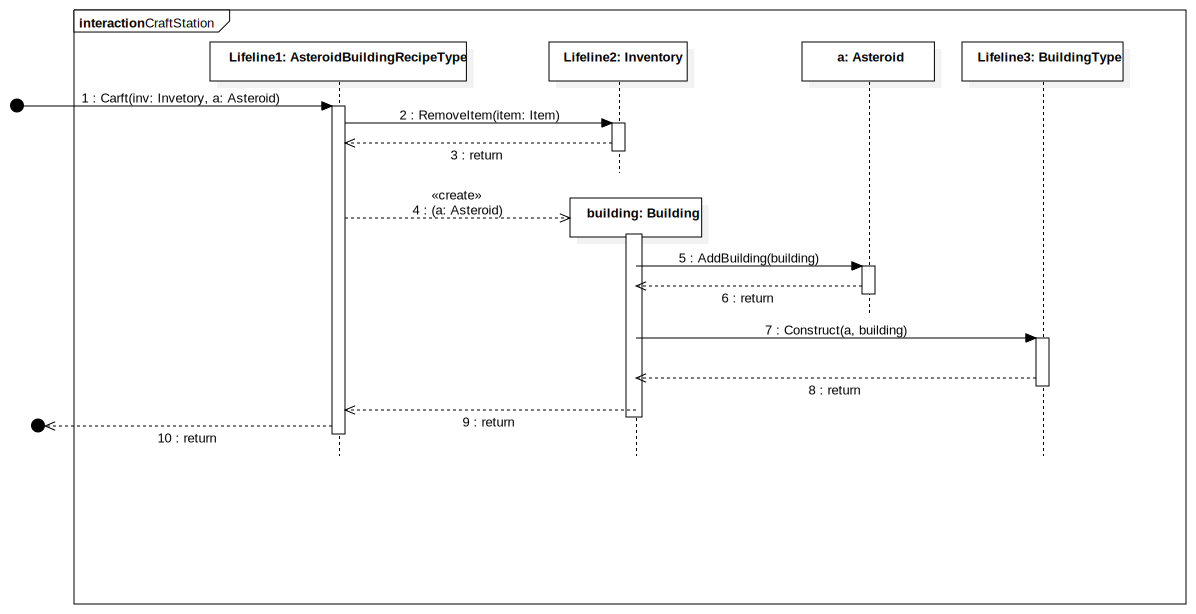
\includegraphics[width=1\textwidth]{docs/2_Project/svg/Design Model!Crafting!Interaction1!CraftStation_20.png}
	\centering
\end{figure}






\begin{figure}[H]
	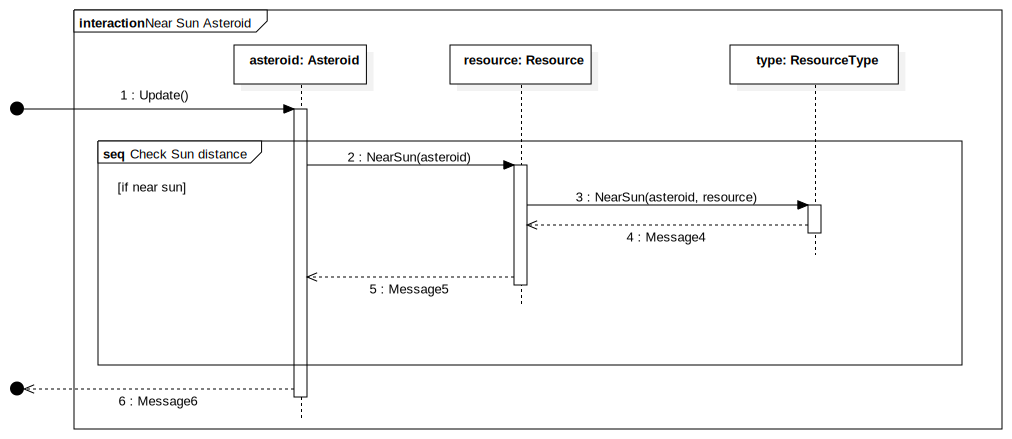
\includegraphics[width=1\textwidth]{docs/2_Project/svg/Design Model!Sun Distance!Asteroid near sun!Near Sun Asteroid_6.png}
	\centering
\end{figure}

\begin{figure}[H]
	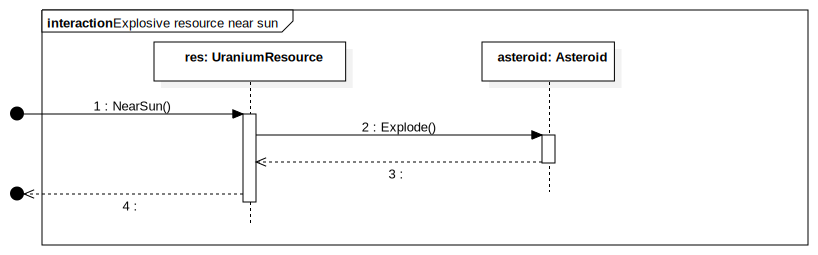
\includegraphics[width=1\textwidth]{docs/2_Project/svg/Design Model!Sun Distance!Resource Explosion!Explosive resource near sun_7.png}
	\centering
\end{figure}

\begin{figure}[H]
	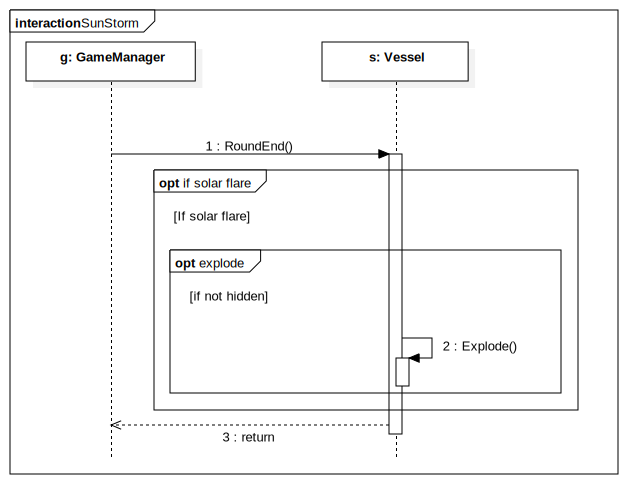
\includegraphics[width=1\textwidth]{docs/2_Project/svg/Design Model!Sun storm!Sun Storm!SunStorm_17.png}
	\centering
\end{figure}

\begin{figure}[H]
	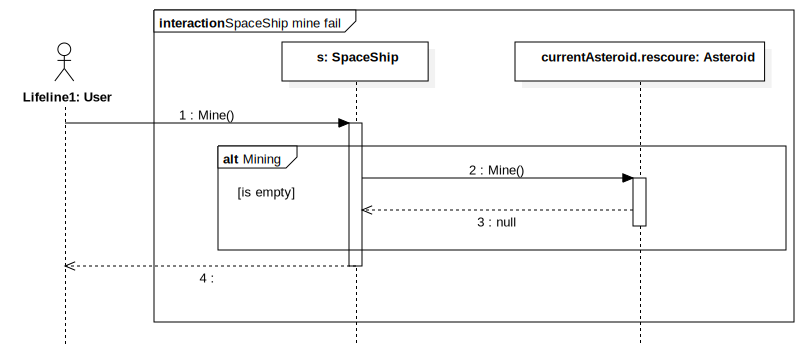
\includegraphics[width=1\textwidth]{docs/2_Project/svg/Design Model!Vessel Actions!SpaceShip mine fail!SpaceShip mine fail_14.png}
	\centering
\end{figure}

\begin{figure}[H]
	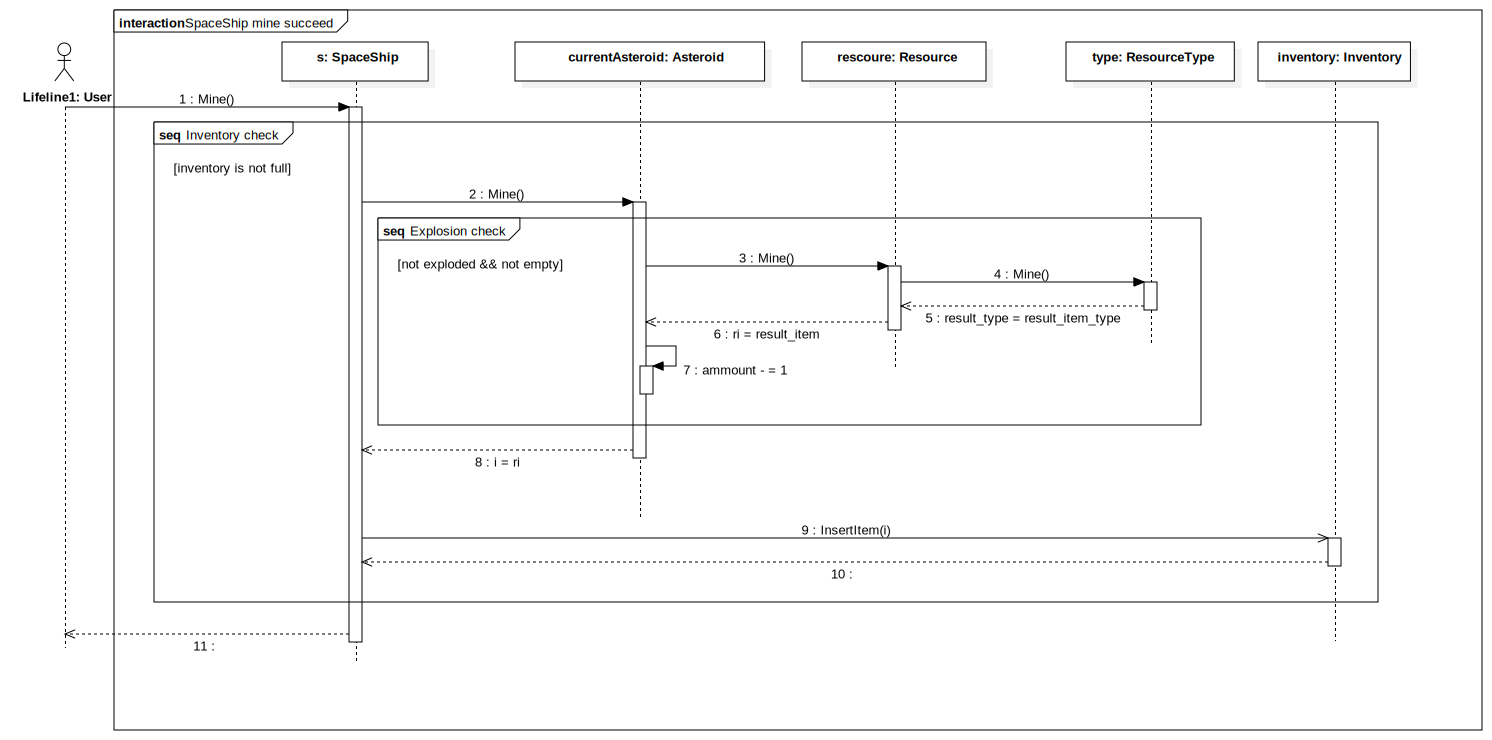
\includegraphics[width=1\textwidth]{docs/2_Project/svg/Design Model!Vessel Actions!SpaceShip mine succeed!SpaceShip mine succeed_13.png}
	\centering
\end{figure}

\begin{figure}[H]
	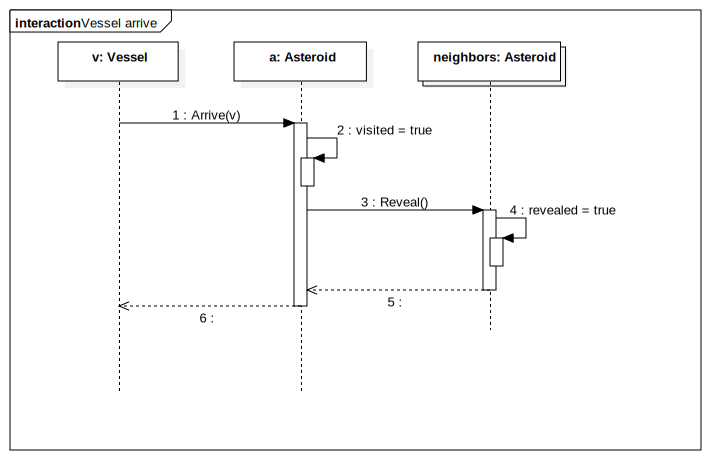
\includegraphics[width=1\textwidth]{docs/2_Project/svg/Design Model!Vessel Actions!Vessel arrive!Vessel arrive_9.png}
	\centering
\end{figure}

\begin{figure}[H]
	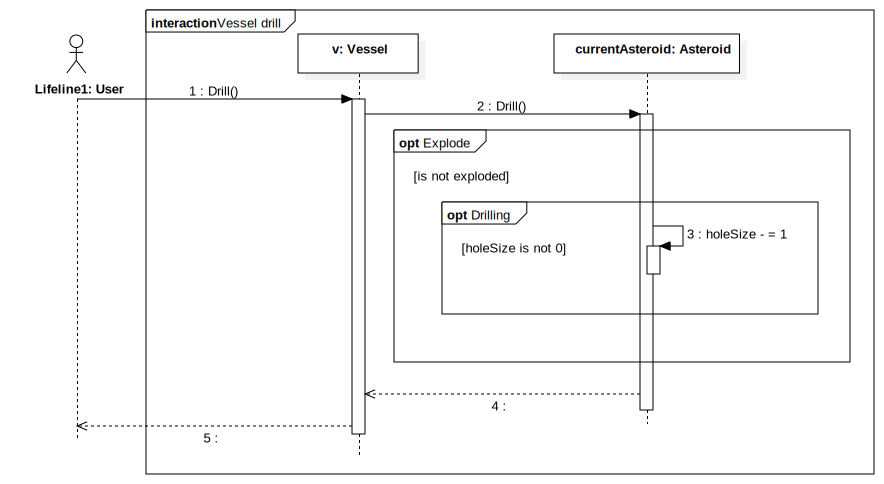
\includegraphics[width=1\textwidth]{docs/2_Project/svg/Design Model!Vessel Actions!Vessel drill!Vessel drill_10.png}
	\centering
\end{figure}

\begin{figure}[H]
	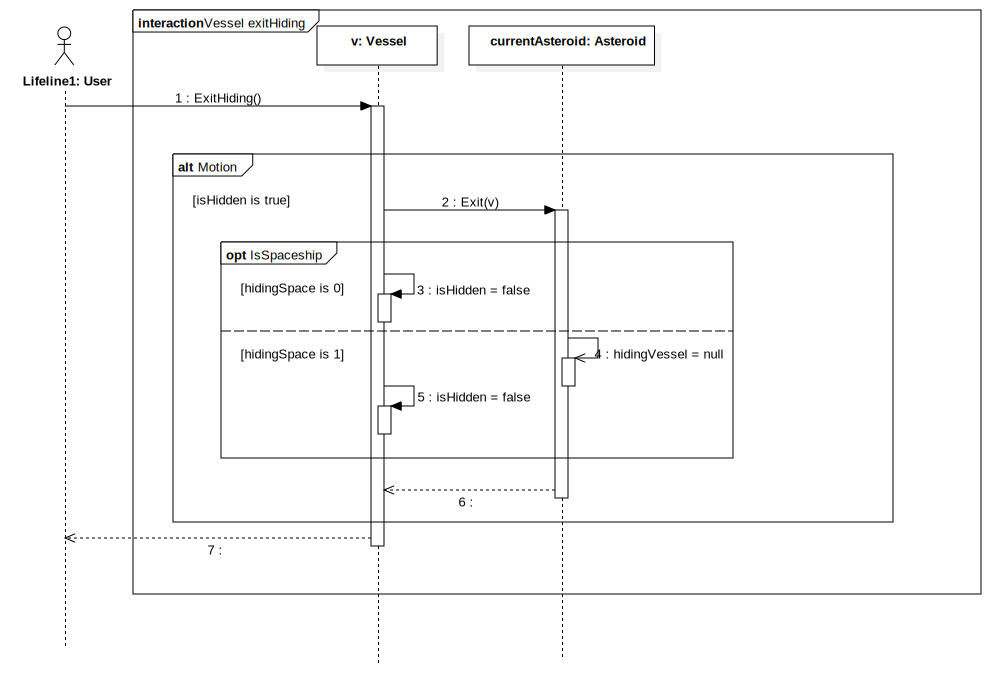
\includegraphics[width=1\textwidth]{docs/2_Project/svg/Design Model!Vessel Actions!Vessel exitHiding!Vessel exitHiding_12.png}
	\centering
\end{figure}

\begin{figure}[H]
	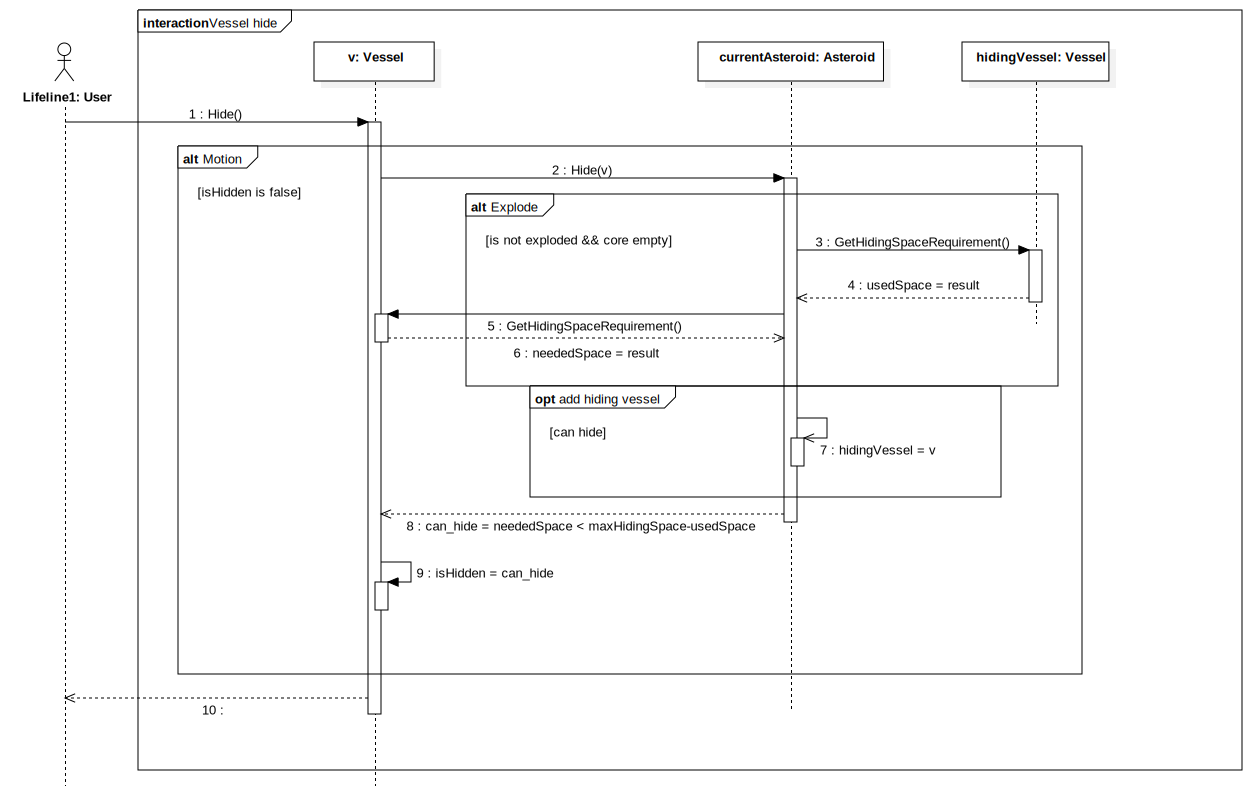
\includegraphics[width=1\textwidth]{docs/2_Project/svg/Design Model!Vessel Actions!Vessel hide!Vessel hide_11.png}
	\centering
\end{figure}

\begin{figure}[H]
	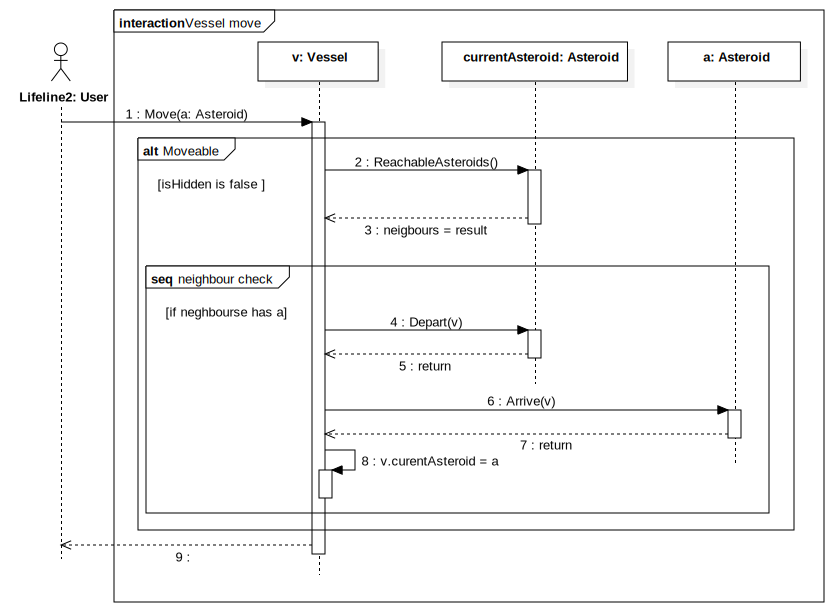
\includegraphics[width=1\textwidth]{docs/2_Project/svg/Design Model!Vessel Actions!Vessel move!Vessel move_8.png}
	\centering
\end{figure}


\section{State-chartok}
%\comment{Csak azokhoz az osztályokhoz, ahol van értelme. Egyetlen állapotból álló state-chartok ne szerepeljenek. A játék működését bemutató state-chart-ot készíteni tilos.}

\begin{figure}[H]
	
\includegraphics[width=1\textwidth]{docs/2_Project/svg/Design Model!NearSun!NearSun_3.png}
	\centering
\end{figure}


\begin{figure}[H]
	
\includegraphics[width=1\textwidth]{docs/2_Project/svg/Design Model!RobotActivities!RobotActivities_4.png}
	\centering
\end{figure}

\begin{figure}[H]
	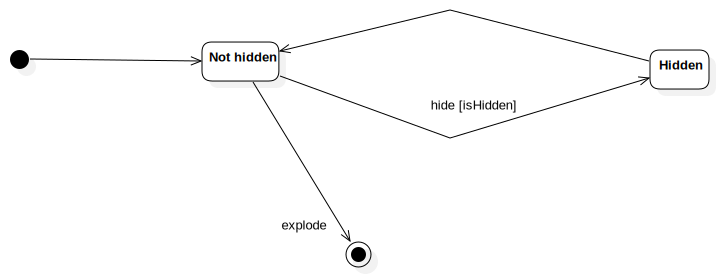
\includegraphics[width=1\textwidth]{docs/2_Project/svg/Design Model!Spaceship Hide!Spaceship Hide_5.png}
	\centering
\end{figure}

\section{Napló}

\begin{naplo}
    \naplotag{2021.02.24. 10:00 }{ 2 óra }{ Csapat }
	{ 
		Konzultációs időpontban csapatmegbeszélés.
        Részletesen: \ref{appendix:meeting4}
	}

    \naplotag{2021.02.26. 17:00 }{ 1 óra }{ Csapat }
	{ 
		Konzultációs időpontban csapatmegbeszélés.
        Részletesen: \ref{appendix:meeting5}
	}
	\naplotag{2021.02.27. 14:00 }{ 3 óra }{ Gao Tong }
	{ 
		Szekvenciák készítése és kisebb javítások a modellben.
        
	}
    \naplotag{2021.02.28. 12:00 }{ 5 óra }{ Nagy Beáta }
	{ 
		Osztálydiagram dokumentáció elkészítése, kérdéses pontok összeírása, megbeszélése a többiekkel.
        
	}
	\naplotag{2021.03.01. 07:00 }{ 3 óra }{ Tatai Titusz }
	{ 
		Szekvenciák készítése és kisebb javítások a modellben.
        
	}
    \naplotag{2021.02.28. 14:00 }{ 2 óra }{ Sike Ádám }
	{ 
		Obkjektum katalógus, és aszteroida sekvencia diagrammok-ban segítség.   
	}

    \naplotag{2021.03.01. 10:00 }{ 4 óra }{ Dömötör Péter }
	{ 
		Dokumentumok összefésülése, Hibák javítása, Osztálydiagram befejezése.   
	}

\end{naplo}

\begin{toappendix}

	\markdownInput[shiftHeadings=2]{\filePath[docs/meetings/meeting-4.md]}

	\markdownInput[shiftHeadings=2]{\filePath[docs/meetings/meeting-5.md]}
	
\end{toappendix}

\end{document}
